\documentclass[10pt,a4paper]{article}
\usepackage[utf8]{inputenc}
\usepackage{amsmath}
\usepackage{amsfonts}
\usepackage{amssymb}
\usepackage{listings}
\usepackage{url}
\usepackage{hyperref}  % autoref
\usepackage{graphicx}  % reflextbox, rotatebox

\lstset{basicstyle=\footnotesize\ttfamily,breaklines=true}
\setlength{\parindent}{0pt}

\begin{document}

Let's look at what the fourier transform of the Gaussian kernel results to:

\begin{align}
\tilde{G}(k)
   := & \mathcal{F}\left[ \tilde{G} \right]
    =   \frac{1}{\sqrt{2\pi}}
        \int\limits_{-\infty}^{\infty} \frac{1}{\sqrt{2\pi}\sigma}
            e^{ \frac{-\left( x - \mu  \right)^2}{2\sigma^2} }
            e^{ \pm \mathrm{i}kx}
        \,\mathrm{d}x \\
    = & \frac{1}{ 2\pi\sigma } e^{-\frac{\mu^2}{2\sigma^2} }
        \int\limits_{-\infty}^{\infty}
            e^{ \frac{ -x^2 + \left(2\mu \pm \mathrm{i}k 2\sigma^2 \right)x}
                    {2\sigma^2} }
        \,\mathrm{d}x \\
    = & \frac{1}{ 2\pi\sigma } e^{-\frac{\mu^2}{2\sigma^2} }
        \int\limits_{-\infty}^{\infty}
            e^{ \frac{ -\left[ x - \left(\mu \pm
                              \mathrm{i}k\sigma^2 \right)
                       \right]^2 +
                       \left(\mu \pm \mathrm{i}k\sigma^2 \right)^2 }
                    {2\sigma^2}
              }
        \,\mathrm{d}x \\
    = & \frac{1}{ 2\pi\sigma } e^{-\frac{\mu^2}{2\sigma^2}}
        e^{\frac{ \mu^2 \pm \mathrm{i} \mu k \sigma^2 -
                  k^2\sigma^4 }{ 2 \sigma^2} }
        \int\limits_{-\infty}^{\infty}
            e^{ \frac{ -\left[ x - \left(\mu \pm
                \mathrm{i}k\sigma^2 \right) \right]^2}{\sigma^2} }
        \,\mathrm{d}x \\
    = & \frac{1}{ 2\pi\sigma }
        e^{ \pm \mathrm{i} \mu k \sigma^2 }
        e^{ -\frac{ k^2\sigma^4 }{ 2 } }
        \sqrt{ 2\pi } \sigma \\
    = & \frac{1}{ \sqrt{2\pi} }
        e^{ \pm \mathrm{i} \mu k \sigma^2  }
        e^{ -\frac{ k^2\sigma^2 }{ 2 } } \\
    = & \sigma e^{ \pm \mathrm{i} \mu k \sigma^2  } G\left( \sigma x \right)
\end{align}

Or by using some basic transformation rules for the fourier transform:

\begin{align}
G(x) := & \frac{1}{\sqrt{2\pi}} e^{ -\frac{ x^2 }{2} } \\
g(k) := & \mathcal{F}\left[ G \right]
   :=   \frac{1}{\sqrt{2\pi}}
        \int\limits_{-\infty}^{\infty} G(x) e^{\mathrm{i} k x} \mathrm{d}x
    =   \frac{1}{\sqrt{2\pi}} \frac{1}{\sqrt{2\pi}}
        \int\limits_{-\infty}^{\infty} e^{\mathrm{i} k x - \frac{ x^2 }{2} }
        \mathrm{d}x \\
    = & \frac{1}{2\pi} \int\limits_{-\infty}^{\infty}
        e^{ - \frac{1}{2} \left( x - \mathrm{i} k \right)^2 +
            \mathrm{i}^2 \frac{ k^2 }{2} } \mathrm{d}x
    =   \frac{1}{2\pi} e^{ - \frac{ k^2 }{2} } \int\limits_{-\infty}^{\infty}
        e^{ - \frac{1}{2} \left( x - \mathrm{i} k \right)^2 } \mathrm{d}x \\
    = & \frac{1}{2\pi} e^{ - \frac{ k^2 }{2} } \sqrt{2\pi}
    =   \frac{1}{ \sqrt{2\pi} } e^{ - \frac{ k^2 }{2} }
    =   G(k) \\
\mathcal{F}\left[G\left( \frac{x-\mu}{\sigma} \right) \right]
    = & \sigma \mathcal{F}\left[G\left( x-\mu \right)\right]\left( \sigma x' \right) \\
    = & \mathcal{F} \left[G\left( \frac{x-\mu}{\sigma} \right) \right]
    =   \sigma e^{ -\mathrm{i} \mu k \sigma^2 } g\left( \sigma x \right) \\
    = & \frac{1}{ \sqrt{2\pi} }
        e^{ \pm \mathrm{i} \mu k \sigma^2  }
        e^{ -\frac{ k^2\sigma^2 }{ 2 } }
\end{align}

Period shifts of the kernel do not influece the convoluted result:
Let $\mathbb{K}$ be $\mathbb{C}$ or $\mathbb{R}$.
%and $L^2\left( \mathbb{K}^2 \right)$ be the space of all Lebesgue-integrable functions on $\mathbb{K}^2$, then:
\begin{align}
T_a : \left( \mathbb{K} \rightarrow \mathbb{K} \right) \rightarrow
      \left( \mathbb{K} \rightarrow \mathbb{K} \right) , \;
      T_a[f](x) \mapsto f(x-a)
\end{align}
Then the translation rule for the Fourier transform can be written as:
\begin{align}
\mathcal{F}\left[ T_a[f] \right]
 = & \frac{1}{ \sqrt{2\pi} }
    \int\limits_{-\infty}^{\infty}
        f(x-a) e^{-\mathrm{i} k x}
    \,\mathrm{d}x \\
 \overset{ y = x-a }{ = } &
    \frac{1}{ \sqrt{2\pi} }
    \int\limits_{-\infty}^{\infty}
        f(y) e^{-\mathrm{i} k (y+a)}
    \,\mathrm{d}x \\
 = & e^{-\mathrm{i} k a}
    \frac{1}{ \sqrt{2\pi} }
    \int\limits_{-\infty}^{\infty}
        f(y) e^{-\mathrm{i} k y}
    \,\mathrm{d}x \\
 = & \frac{1}{ \sqrt{2\pi} } e^{-\mathrm{i} k a} \mathcal{F}\left[ f \right]
\end{align}
Here we define the function (not a functional) $\tilde{T}_a(k)$ which shifts in real space $x$ when multiplied with a function in frequency-space $k$:
\begin{align}
    \tilde{T}_a(k) := & \frac{1}{ \sqrt{2\pi} } e^{-\mathrm{i} k a} \\
    \mathcal{F}\left[ \tilde{T}_a \right](x)
    = & T_a\left[ \delta \right](x)
    =   \delta\left( x-a \right) \\
    \mathcal{F}^{-1}\left[ \tilde{T}_a \right](x)
    = & T_{-a}\left[ \delta \right](x)
    =   \delta\left( x+a \right) \\
\end{align}
Function are to be equal if $\forall x: f(x) = g(x)$.
With this we can take a closer look at shifted kernels $G$:
\begin{align}
    f \ast T_a[G]
    = & \mathcal{F}^{-1}\left[
          \mathcal{F}\left[ f \right] \cdot
          \mathcal{F}\left[ T_a[G] \right]
      \right] \\
    = & \mathcal{F}^{-1}\left[
          \mathcal{F}\left[ f \right] \cdot
          \tilde{T}_a \cdot
          \mathcal{F}\left[ G \right]
      \right] \\
    = & \mathcal{F}^{-1}\left[
          \mathcal{F}\left[ T_a[f] \right] \cdot
          \mathcal{F}\left[ G \right]
      \right] \\
    = & T_a[f] \ast G
\end{align}
This means if we blur an image with a kernel which is shifted, then the resulting blurred image will be shifted, too.
This means we need to create the Gaussian at $x=0,y=0$.
For the FFTW-Library the 2D array is expected to lie in memory in row-major format, i.e. the coordinate \lstinline!(ix,iy)! is at \lstinline!data[iy*Nx+ix]!.
This means the center of the Gaussian is at \lstinline!data[0]\lstinline! and the four nearest and therefore highest-value neighbors are at \lstinline!data[1]!, \lstinline!data[Nx]!, \lstinline!data[(Ny-1)*Nx]!, \lstinline!data[(Ny-1)*Nx+Nx-1]!.
In this and only this case the Fourier transform of a real Gaussian kernel will also be a real Gaussian, as seen above. This can be used by checking if the transformed kernel has no imaginary part.


ToDo:
\begin{itemize}
    \item Be more rigorous about $2\pi$ factors in convulation theorem
    \item Relate results for Fourier Transform to the actually used Discrete Fourier Transform \url{https://en.wikipedia.org/wiki/Discrete_Fourier_transform#Circular_convolution_theorem_and_cross-correlation_theorem}
    Basically everything we used, like the translation or convultion theorem also exist for the DFT, therefore the proofs above also hold true for the DFT.
\end{itemize}


\begin{figure}
    \begin{center}\begin{minipage}{0.5\linewidth}
    \begin{minipage}{0.5\linewidth}\begin{center}
        Image to blur
    \end{center}\end{minipage}\begin{minipage}{0.5\linewidth}\begin{center}
        Gaussian kernel
    \end{center}\end{minipage}
    \begin{minipage}{0.5\linewidth}\begin{center}
        \reflectbox{\rotatebox[origin=c]{180}{
\includegraphics[width=\linewidth]{toBlur.png}}}
    \end{center}\end{minipage}\begin{minipage}{0.5\linewidth}\begin{center}
        \reflectbox{\rotatebox[origin=c]{180}{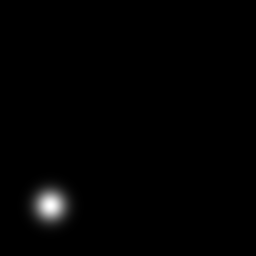
\includegraphics[width=\linewidth]{extendedKernel.png}}}
    \end{center}\end{minipage}\begin{center}
            $\downarrow \mathcal{F}$
    \end{center}\begin{minipage}{0.5\linewidth}
        \reflectbox{\rotatebox[origin=c]{180}{
\includegraphics[width=\linewidth]{toBlurFt.png}}}
    \end{minipage}\begin{minipage}{0.5\linewidth}\begin{center}
        \reflectbox{\rotatebox[origin=c]{180}{
\includegraphics[width=\linewidth]{extendedKernelFt.png}}}
    \end{center}\end{minipage}\begin{center}
                $\downarrow$\\
        periodically cycle images and also use log-scale for better viewing
    \end{center}\begin{minipage}{0.5\linewidth}
        \reflectbox{\rotatebox[origin=c]{180}{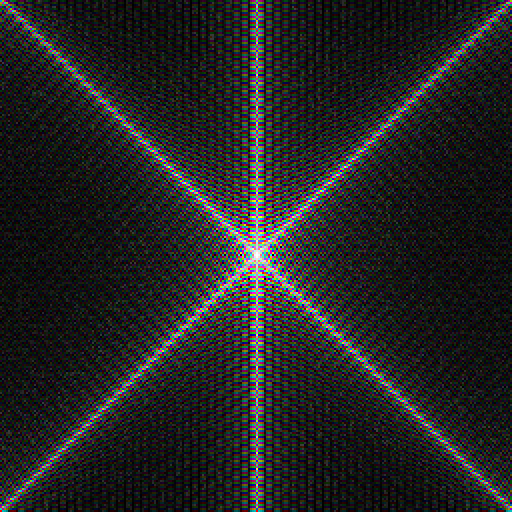
\includegraphics[width=\linewidth]{toBlurFtSwapped.png}}}
    \end{minipage}\begin{minipage}{0.5\linewidth}\begin{center}
        \reflectbox{\rotatebox[origin=c]{180}{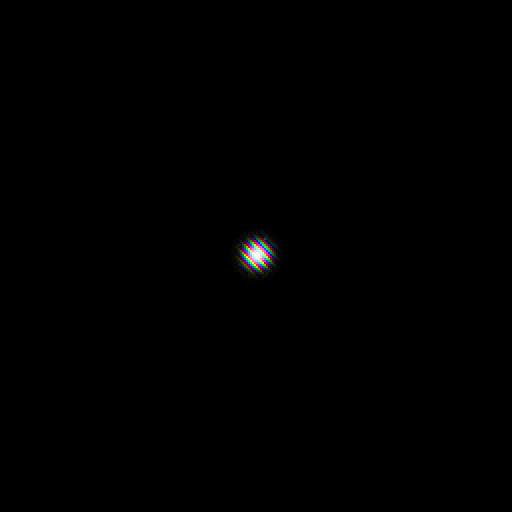
\includegraphics[width=\linewidth]{extendedKernelFtSwapped.png}}}
    \end{center}\end{minipage}\begin{center}
            $\downarrow$\\
        Multiply complex numbers cell-wise
    \end{center}\begin{center}\begin{minipage}{0.5\linewidth}\begin{center}
        \reflectbox{\rotatebox[origin=c]{180}{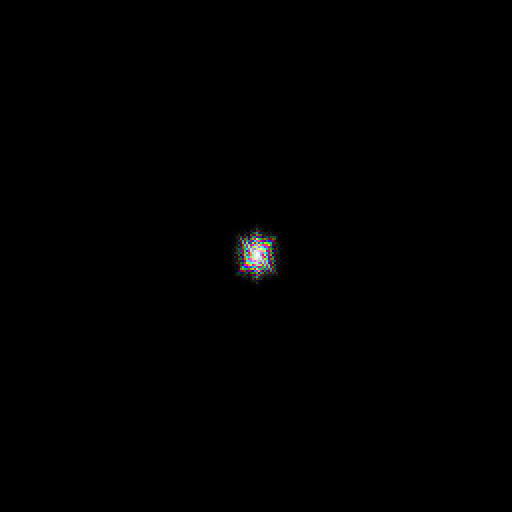
\includegraphics[width=\linewidth]{multiplied.png}}}
    \end{center}\end{minipage}\\
        $\downarrow \mathcal{F}^{-1}$\\
    \begin{minipage}{0.5\linewidth}\begin{center}
        \reflectbox{\rotatebox[origin=c]{180}{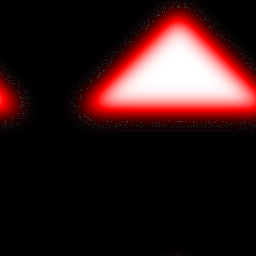
\includegraphics[width=\linewidth]{blurred.png}}}
    \end{center}\end{minipage}\end{center}
    \end{minipage}\end{center}
    \caption{Exemplary blurring of a $256 \times 256$ large image containing a triangle with a Gaussian with $\sigma=10$ at position $(50,50)$.}
    \label{fig:blurring}
\end{figure}

Initially the kernel and the input image in \autoref{fig:blurring} are black and white images with pixels in $[0.0,1.0]$, but after the first transform they are always complex valued.
The complex values are visualized with the magnitude as luminosity and the phase being converted to a hue.
A zero phase, i.e. a real value, maps to a red hue.
Note that perfect white can't be colored with the hue in the HSL-scheme, therefore the phase information can't be plotted inside the triangle.
It can be seen, that the resulting blurred image has some very small non-zero phases, because of numerical errors.

As can be seen, because the Gaussian kernel is not perfect at $(x,y)=(0,0)$, but at $(50,50)$ the triangle gets shifted.
This means the kernel must be at zero, which is the upper left corner which corresponds to the very first value in the linearized 1D array of complex values as FFTW or cuFFT uses it.

\end{document}
